\documentclass[11pt,a4paper,parskip=half,DIV=12,headinclude,footinclude]{scrartcl}

% --- Typography: Inter remains the only document typeface ---
\usepackage{fontspec}
\usepackage[french]{babel}
\usepackage{microtype}
\usepackage[table]{xcolor}
\usepackage{booktabs}
\usepackage{tabularx}
\usepackage{graphicx}
\usepackage{setspace}
\usepackage{listings}
\usepackage{hyperref}
\usepackage{scrlayer-scrpage}
\usepackage{enumitem}
\usepackage{needspace}
\usepackage{tikz}

\setmainfont{Inter}[
  Path           = fonts/,
  Extension      = .ttf,
  UprightFont    = *-Regular,
  BoldFont       = *-Bold,
  ItalicFont     = *-Regular,
  BoldItalicFont = *-Bold,
]

\DeclareFontShape{TU}{Inter(0)}{b}{sc}{<-> ssub*Inter(0)/b/n}{}

% --- Restrained visual identity ---
\definecolor{ink}{HTML}{17212B}
\definecolor{muted}{HTML}{667482}
\definecolor{brand}{HTML}{C46A45}
\definecolor{branddark}{HTML}{914A31}
\definecolor{brandsoft}{HTML}{F8EEE9}
\definecolor{codebg}{HTML}{F3F6F8}
\definecolor{rulecolor}{HTML}{DCE4E8}
\definecolor{paperwhite}{HTML}{FFFFFF}

% --- KOMA-Script typography ---
\setkomafont{title}{\bfseries\fontsize{34}{39}\selectfont\color{ink}}
\setkomafont{subtitle}{\mdseries\fontsize{13}{18}\selectfont\color{muted}}
\setkomafont{author}{\small\color{ink}}
\setkomafont{date}{\small\color{muted}}
\setkomafont{section}{\bfseries\Large\color{ink}}
\setkomafont{subsection}{\bfseries\large\color{ink}}
\setkomafont{caption}{\small\upshape\color{muted}}
\setkomafont{captionlabel}{\bfseries\upshape\color{branddark}}

\renewcommand*{\sectionformat}{\textcolor{brand}{\thesection\autodot}\enskip}
\renewcommand*{\subsectionformat}{\textcolor{brand}{\thesubsection\autodot}\enskip}

\RedeclareSectionCommand[
  beforeskip=2.0em,
  afterskip=0.75em,
  afterindent=false
]{section}
\RedeclareSectionCommand[
  beforeskip=1.25em,
  afterskip=0.45em,
  afterindent=false
]{subsection}

% --- Page rhythm and whitespace ---
\setlength{\parindent}{0pt}
\setlength{\parskip}{0.55em}
\setlength{\emergencystretch}{3em}
\setstretch{1.13}
\renewcommand{\arraystretch}{1.3}
\setlength{\tabcolsep}{9pt}
\setlength{\textfloatsep}{1.4em plus 0.3em minus 0.2em}
\setlength{\intextsep}{1.2em plus 0.3em minus 0.2em}
\setlength{\abovecaptionskip}{0.55em}
\setlength{\belowcaptionskip}{0.2em}
\setlength{\fboxsep}{7pt}
\setlength{\fboxrule}{0.4pt}

\graphicspath{{../screenshots/}}
\urlstyle{same}
\addto\captionsfrench{\renewcommand{\tablename}{Tableau}}

% --- Running header and footer ---
\clearpairofpagestyles
\ihead{\small\color{muted}CITYTRACE}
\ohead{\small\color{muted}Rapport de mini-projet}
\setheadsepline{0.4pt}
\setfootsepline{0pt}
\cfoot{\small\color{muted}\pagemark}
\setkomafont{pagehead}{\normalfont}
\setkomafont{pagefoot}{\normalfont}
\pagestyle{scrheadings}

% --- Tables ---
\renewcommand{\arraystretch}{1.3}
\newcommand{\tableheadstyle}{\rowcolor{brandsoft}\color{ink}\color{ink}}

% --- Code listings ---
\lstset{
  basicstyle=\ttfamily\footnotesize\color{ink},
  backgroundcolor=\color{codebg},
  frame=single,
  rulecolor=\color{rulecolor},
  framesep=0.8em,
  framerule=0.4pt,
  xleftmargin=0pt,
  xrightmargin=0pt,
  breaklines=true,
  columns=fullflexible,
  keepspaces=true,
  showstringspaces=false,
  aboveskip=0.9em,
  belowskip=0.9em,
  keywordstyle=\bfseries\color{branddark},
  commentstyle=\itshape\color{muted},
  morekeywords={revert,emit,uint8,Status,internal,pure,returns},
}

% --- Links and PDF metadata ---
\hypersetup{
  colorlinks=true,
  linkcolor=branddark,
  urlcolor=branddark,
  citecolor=branddark,
  pdftitle={CityTrace --- Registre de signalements urbains},
  pdfauthor={Yassir Hannaoui},
  pdfsubject={Rapport de mini-projet},
  pdfcreator={LaTeX}
}

% Keep figures visually contained without changing their source images.
\let\originalincludegraphics\includegraphics
\newsavebox{\citytraceimagebox}
\renewcommand{\includegraphics}[2][]{%
  \begingroup
  \sbox{\citytraceimagebox}{\originalincludegraphics[#1]{#2}}%
  \begin{tikzpicture}
    \clip[rounded corners=9pt]
      (0,0) rectangle
      (\wd\citytraceimagebox,\dimexpr\ht\citytraceimagebox+\dp\citytraceimagebox\relax);
    \node[anchor=south west,inner sep=0pt] at (0,0)
      {\usebox{\citytraceimagebox}};
  \end{tikzpicture}%
  \endgroup
}

\title{CityTrace}
\subtitle{Registre de signalements urbains --- rapport de mini-projet}
\author{Yassir Hannaoui}
\date{Novembre 2026}

\begin{document}

\maketitle
\vspace{-0.65em}
\noindent{\color{brand}\rule{\textwidth}{1.6pt}}
\vspace{0.7em}

\begin{quote}
\small\color{muted}
    \url{https://github.com/MadMax-5000/blockchain}
\end{quote}
\vspace{0.3em}

\section{Le point de départ}

Un lampadaire qui clignote, un trottoir effondré, une poubelle pleine : le
signalement part souvent d'un message envoyé nulle part, puis d'une relance par
téléphone. J'ai voulu une trace unique, du premier dépôt jusqu'à la clôture, que
le citoyen et la municipalité puissent lire sans se faire confiance. Elle tient
dans un seul contrat Solidity, \texttt{UrbanIssueRegistry}. L'interface React ne
stocke rien : elle lit le contrat et signe les écritures avec MetaMask.

Chaque fiche porte neuf champs : identifiant, type, lieu, description, date,
priorité, déclarant, équipe affectée et statut. Les huit dossiers du jeu de
démonstration utilisent des pseudonymes (\texttt{Citizen01},
\texttt{UrbanTeam01}) et des quartiers fictifs. Aucune donnée personnelle réelle
n'entre dans le contrat.

\section{Une chaîne, pas un bouton \og{}terminé\fg{}}

Le statut n'est pas un champ libre. Il avance d'une case à la fois :
\texttt{Signalé} $\to$ \texttt{Affecté} $\to$ \texttt{En cours} $\to$
\texttt{Résolu} $\to$ \texttt{Clôturé}. \texttt{assignTeam} est la porte d'entrée
dans \texttt{Affecté} : elle écrit l'équipe et l'historique dans la même
transaction. Ensuite, \texttt{updateStatus} vérifie la transition dans le
contrat, pas dans le React.

\begin{lstlisting}
function _isValidTransition(Status from, Status to) internal pure returns (bool) {
    if (from == Status.Reported)   return to == Status.Assigned;
    if (from == Status.Assigned)   return to == Status.InProgress;
    if (from == Status.InProgress) return to == Status.Resolved;
    if (from == Status.Resolved)   return to == Status.Closed;
    return false;
}
\end{lstlisting}

Un appel direct qui demanderait \texttt{Resolved} depuis \texttt{InProgress} est
donc rejeté avec \texttt{InvalidStatusTransition}. Le bouton
\og{}Passer à\ldots{}\fg{} de l'espace municipal ne propose que l'étape suivante ;
c'est un confort d'interface, la règle est celle ci-dessus. Une équipe ne peut
plus être changée après \texttt{Résolu}.

\begin{figure}[htbp]
\centering
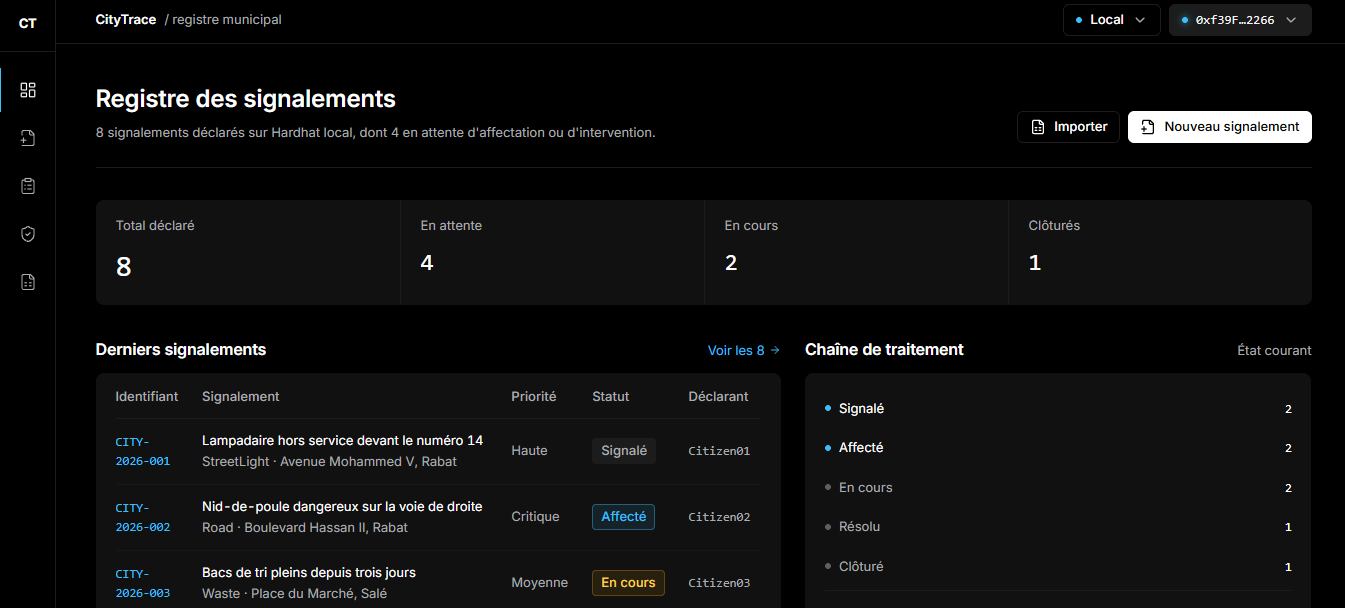
\includegraphics[width=\textwidth]{Registre des signalements}
\caption{L'accueil. Les compteurs viennent de la lecture des fiches et la
colonne de droite montre la répartition par statut.}
\end{figure}

\section{Deux portes d'entrée}

Le formulaire citoyen est volontairement court. Il ne décide que du contenu de
la fiche : le contrat impose \texttt{Reported} au moment de la création. La
transaction est signée dans MetaMask, le frontend attend le reçu, puis il
invalide son cache de lecture. Le dossier apparaît ensuite en tête de liste,
sans aucune étape municipale prématurée.

\begin{figure}[htbp]
\centering
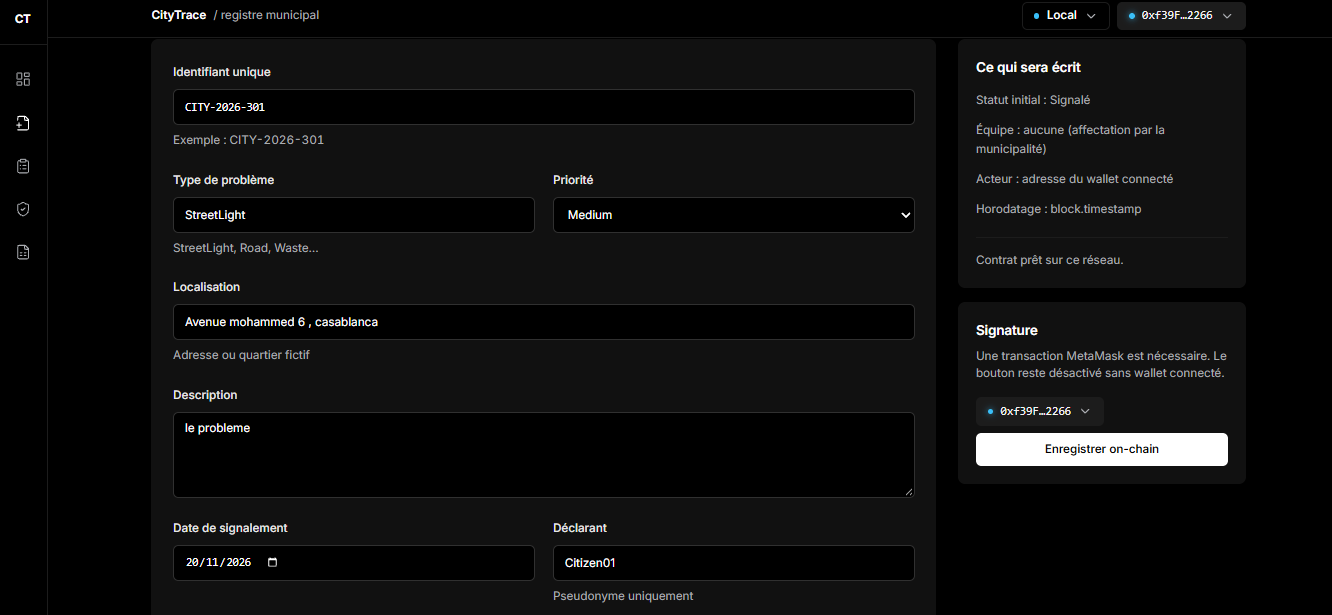
\includegraphics[width=\textwidth]{nouveau-signalement}
\caption{Le formulaire de déclaration. Le déclarant choisit le type, le lieu,
la date et la priorité ; le statut initial, lui, n'est pas un champ du formulaire.}
\end{figure}

Pour une campagne municipale, ce formulaire serait ridicule. L'import Excel lit
le classeur dans le navigateur avec SheetJS, puis contrôle les neuf colonnes
attendues, les dates, les énumérations, les doublons du fichier et ceux déjà
présents on-chain. Les lignes fautives sont signalées et ne peuvent pas être
cochées. Un lot est limité à 50~lignes et demande \texttt{AGENT\_ROLE}.
\texttt{batchCreateIssues} est atomique : un seul identifiant déjà utilisé
annule tout le lot. Deux classeurs accompagnent la démo, l'un avec 8~lignes
propres, l'autre avec 10~lignes dont 5~erreurs volontaires.

\begin{figure}[htbp]
\centering
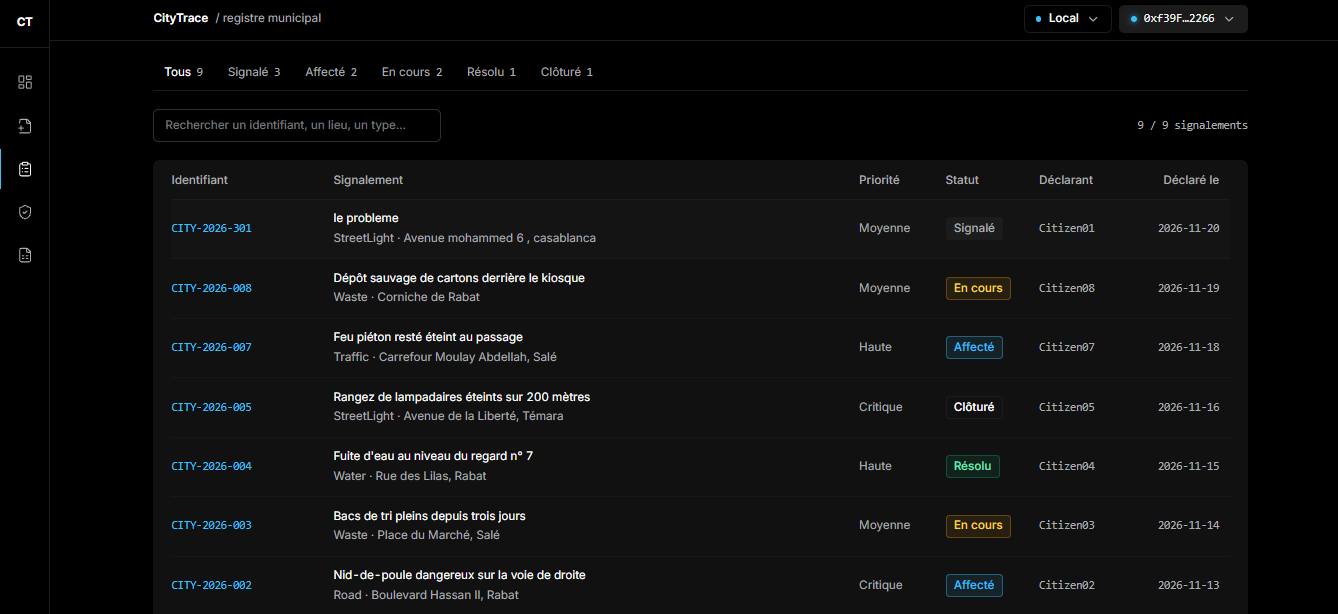
\includegraphics[width=\textwidth]{Signalements}
\caption{La liste publique. Filtres par statut et recherche textuelle fonctionnent
sans wallet connecté ; seules les actions d'agent demandent une signature.}
\end{figure}

\section{Le wallet ne sert qu'à signer}

Les routes \texttt{/}, \texttt{/issues} et \texttt{/issues/:issueId} passent par
le RPC local : la consultation est ouverte. Dès qu'une écriture est demandée ---
affectation, changement de statut, import, pause --- MetaMask signe avec le
compte municipal. Sur le nœud de référence, le déployeur est le compte~\#0 de
Hardhat, \texttt{0xf39Fd6e51aad88F6F4ce6aB8827279cffFb92266}. Le constructeur
lui donne les deux rôles suivants.

\begin{table}[htbp]
\centering
\caption{Deux rôles suffisent pour la démonstration.}
\begin{tabularx}{\textwidth}{@{}lX@{}}
\toprule
\rowcolor{brandsoft}\color{ink}
\textbf{Rôle} & \textbf{Ce qu'il autorise} \\
\midrule
\texttt{AGENT\_ROLE} & affecter une équipe, avancer le statut, importer un lot \\
\texttt{DEFAULT\_ADMIN\_ROLE} & mettre en pause, reprendre, accorder ou retirer un rôle \\
\bottomrule
\end{tabularx}
\end{table}

Les erreurs du contrat sont traduites dans l'interface : doublon, rôle manquant,
mauvais réseau, transition interdite, contrat en pause, lot trop grand. Le hash
de transaction est affiché avec un bouton de copie. Sur une chaîne publique, un
lien vers l'explorateur serait ajouté ; sur le réseau local je n'en fabrique pas.

\section{Ce que j'ai vérifié}

Le déploiement de référence tourne sur Hardhat local, chainId~31337. Le registre
est au bloc~1, à l'adresse
\texttt{0x5FbDB2315678afecb367f032d93F642f64180aa3}. La clé privée du compte~\#0
est celle fournie par Hardhat ; elle ne sert qu'à cette démo et n'apparaît
nulle part dans le frontend.

\begin{table}[htbp]
\centering
\caption{Relevés sur le nœud local de référence.}
\begin{tabularx}{\textwidth}{@{}lXl@{}}
\toprule
\rowcolor{brandsoft}\color{ink}
\textbf{Commande} & \textbf{Contrôle} & \textbf{Résultat} \\
\midrule
\texttt{npm test} & rôles, doublons, transitions, lots, pause, événements & \textbf{31 passing} \\
\texttt{smoke:local} & comptages et historique de \texttt{CITY-2026-005} & 8 dossiers, 5 entrées \\
\texttt{typecheck} & \texttt{tsc --noEmit} & aucune erreur \\
\texttt{build} & compilation Vite de production & OK \\
inspecteur & 1440 / 768 / 390~px & 0~FAIL \\
\bottomrule
\end{tabularx}
\end{table}

Les 8~signalements créés par le script \texttt{seed.ts} produisent
8~\texttt{IssueCreated}, 6~\texttt{IssueAssigned} et
13~\texttt{IssueStatusUpdated}. Le dossier \texttt{CITY-2026-005} est clos et
porte cinq entrées d'historique horodatées. Le build de production a aussi été
ouvert dans un navigateur aux trois largeurs : aucun débordement ni avertissement
de mise en page.

\end{document}
